\documentclass{llncs}
%%%%%%%%%%%%%%%%%%%%%%%%%%%%%%%%%%%%%%%%%%%%%%%%%%%%%%%%%%%
%% package sillabazione italiana e uso lettere accentate
\usepackage[latin1]{inputenc}
\usepackage[english]{babel}
\usepackage[T1]{fontenc}

\usepackage{listings}

%%%%%%%%%%%%%%%%%%%%%%%%%%%%%%%%%%%%%%%%%%%%%%%%%%%%%%%%%%%%%

\usepackage{url}
\usepackage{xspace}

\usepackage{float}

\makeatletter
%%%%%%%%%%%%%%%%%%%%%%%%%%%%%% User specified LaTeX commands.
\usepackage{manifest}

\makeatother


%%%%%%%
 \newif\ifpdf
 \ifx\pdfoutput\undefined
 \pdffalse % we are not running PDFLaTeX
 \else
 \pdfoutput=1 % we are running PDFLaTeX
 \pdftrue
 \fi
%%%%%%%
 \ifpdf
 \usepackage[pdftex]{graphicx}
 \else
 \usepackage{graphicx}
 \fi
%%%%%%%%%%%%%%%
 \ifpdf
 \DeclareGraphicsExtensions{.pdf, .jpg, .tif}
 \else
 \DeclareGraphicsExtensions{.eps, .jpg}
 \fi
%%%%%%%%%%%%%%%
 
\newcommand{\java}{\textsf{Java}}
\newcommand{\contact}{\emph{Contact}}
\newcommand{\corecl}{\texttt{corecl}}
\newcommand{\medcl}{\texttt{medcl}}
\newcommand{\msgcl}{\texttt{msgcl}}
\newcommand{\android}{\texttt{Android}}
\newcommand{\dsl}{\texttt{DSL}}
\newcommand{\jazz}{\texttt{Jazz}}
\newcommand{\rtc}{\texttt{RTC}}
\newcommand{\ide}{\texttt{Contact-ide}}
\newcommand{\xtext}{\texttt{XText}}
\newcommand{\xpand}{\texttt{Xpand}}
\newcommand{\xtend}{\texttt{Xtend}}
\newcommand{\pojo}{\texttt{POJO}}
\newcommand{\junit}{\texttt{JUnit}}

\newcommand{\action}[1]{\texttt{#1}\xspace}
\newcommand{\code}[1]{{\small{\texttt{#1}}}\xspace}
\newcommand{\codescript}[1]{{\scriptsize{\texttt{#1}}}\xspace}

% Cross-referencing
\newcommand{\labelsec}[1]{\label{sec:#1}}
\newcommand{\xs}[1]{\sectionname~\ref{sec:#1}}
\newcommand{\xsp}[1]{\sectionname~\ref{sec:#1} \onpagename~\pageref{sec:#1}}
\newcommand{\labelssec}[1]{\label{ssec:#1}}
\newcommand{\xss}[1]{\subsectionname~\ref{ssec:#1}}
\newcommand{\xssp}[1]{\subsectionname~\ref{ssec:#1} \onpagename~\pageref{ssec:#1}}
\newcommand{\labelsssec}[1]{\label{sssec:#1}}
\newcommand{\xsss}[1]{\subsectionname~\ref{sssec:#1}}
\newcommand{\xsssp}[1]{\subsectionname~\ref{sssec:#1} \onpagename~\pageref{sssec:#1}}
\newcommand{\labelfig}[1]{\label{fig:#1}}
\newcommand{\xf}[1]{\figurename~\ref{fig:#1}}
\newcommand{\xfp}[1]{\figurename~\ref{fig:#1} \onpagename~\pageref{fig:#1}}
\newcommand{\labeltab}[1]{\label{tab:#1}}
\newcommand{\xt}[1]{\tablename~\ref{tab:#1}}
\newcommand{\xtp}[1]{\tablename~\ref{tab:#1} \onpagename~\pageref{tab:#1}}
% Category Names
\newcommand{\sectionname}{Section}
\newcommand{\subsectionname}{Subsection}
\newcommand{\sectionsname}{Sections}
\newcommand{\subsectionsname}{Subsections}
\newcommand{\secname}{\sectionname}
\newcommand{\ssecname}{\subsectionname}
\newcommand{\secsname}{\sectionsname}
\newcommand{\ssecsname}{\subsectionsname}
\newcommand{\onpagename}{on page}

\newcommand{\xauthA}{Roberto Casadei}
\newcommand{\xauthB}{NameB StudentB}
\newcommand{\xauthC}{NameC StudentC}
\newcommand{\xfaculty}{II Faculty of Engineering}
\newcommand{\xunibo}{Alma Mater Studiorum -- University of Bologna}
\newcommand{\xaddrBO}{viale Risorgimento 2}
\newcommand{\xaddrCE}{via Venezia 52}
\newcommand{\xcityBO}{40136 Bologna, Italy}
\newcommand{\xcityCE}{47023 Cesena, Italy}

%
% Comments
%
\newcommand{\todo}[1]{\bf{TODO:}\emph{#1}}

\setcounter{secnumdepth}{3}
\setcounter{tocdepth}{3}

\begin{document}

\title{Convoy Cruise Control}

\author{\xauthA}

\institute{%
  \xunibo\\\xaddrCE, \xcityCE\\\email{roberto.casadei12@studio.unibo.it}
}

\maketitle

\begin{abstract}
\footnotesize
This document represents a snapshot of the development process of the Convoy Cruise Control.

%MANIFEST
%\category{I.2.5}{Artificial Intelligence}{Programming Languages and Software}
%\category{I.2.11}{Artificial Intelligence}{Distributed Artificial Intelligence}[Intelligent Agents]

%\terms{Agent programming languages; Methodologies and Languages}

%\keywords{Environment programming in Multi-Agent Systems, Action/perception models, Agent Programming Languages}

\keywords{Convoy Cruise Control, control system, development process, requirements, analysis, project, implementation, testing.}
\end{abstract}

\sloppy

%===========================================================================
\section{Introduction}
\labelsec{intro}
%===========================================================================

\subsection{Vision}
In case of environmental disasters, the technology can help.\\
In particular, the need of tools and goods is prominent.\\
A convoy of vehicles can satisfy this need. 
Moreover, it would be great if we were able to reckon on a control system in order to ease the management of the convoy.

\subsection{Goals}
We would like to develop the software support which will be installed onto the vehicles and on the chief vehicle. All this software forms what we call the \emph{Convoy Cruise Control} system.\\
As it is a software project, we will apply the principles of software engineering in order to reduce the time and cost of the project.\\
Our aim is to apply a software process that is repeatable, defined and managed.

%===========================================================================
\section{Requirements}
\labelsec{Requirements}
%===========================================================================

Look at \url{www.cruisecontrolsystem.it/requirements.pdf}

%===========================================================================
\section{Requirement analysis}
\labelsec{ReqAnalysis}
%===========================================================================



\subsection{Glossary}
\begin{itemize}
  \item \emph{CONVOY CRUISE CONTROL}: It is a control system that allows to manage the convoy and the convoy's vehicles. It receives the information from the vehicles about their status and speed, and send commands to them, allowing to monitor and control the behavior of the overall convoy and of the single vehicles.\\

  \item \emph{CONVOY}: It is a line of vehicles with a chief at the head.\\

  \item \emph{VEHICLE}: It is a means of conveyance which is able to move autonomously. It must keep a precise position in the line and move at the \emph{speed} which has been set by the chief. It includes a dashboard with a display that shows the current speed (in Kms/sec and Kms/h) and the number of kilometers covered by the vehicle.\\

  \item \emph{CHIEF VEHICLE}: It is the vehicle on which the chief (the person responsible for the convoy) stays. It has a dashboard which is composed of a display that shows the status of all the convoy's vehicles and of a display like that of the other vehicles. Moreover, the chief vehicles has a control panel that allows to set the convoy speed and to make it start and stop. Through the dashboard and the control panel, the chief can interface himself to the Cruise Control System. \\

  \item \emph{DASHBOARD}: It is a panel that contains displays which allow to see multiple information. \\

  \item \emph{DISPLAY}: It is something that can render some textual content.\\

  \item \emph{CONTROL PANEL}: It is a panel which contains buttons and input fields. It allows to send commands to the convoy's vehicles upon a certain communication infrastructure.\\

  \item \emph{KILOMETER COUNTER}: It's needed by the vehicles in order to keep the count of the kilometers covered.\\
\end{itemize}

\newpage

\subsection{Use Cases}

\begin{figure}
   \centering
   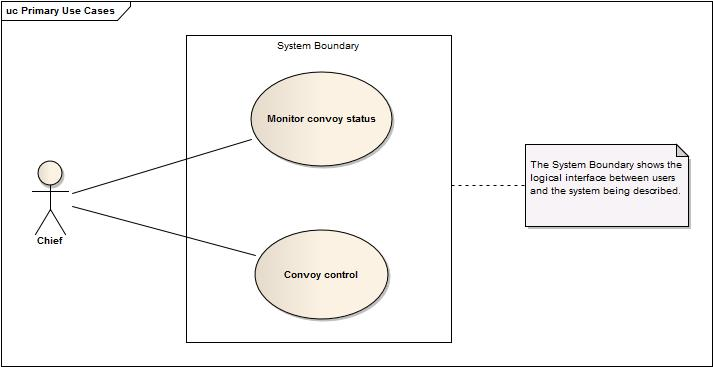
\includegraphics[scale = 0.5]{../Diagrams/Primary_Use_Cases.jpg}\\
  \caption{Primary use cases}\labelfig{testTypes}
\end{figure}

\subsection{Scenarios}
The following scenarios express the main things we want the system to do. 

\begin{table}[H]
\caption{Scenario 1: Monitor Convoy Status}
\label{tab:Scenario1}
\begin{tabular}{| p{2cm} | p{10cm} |}
\hline
\bf{Field} & \bf{Description}\\[3pt]
\hline
ID(Nome) & UC1 - Monitor Convoy Status\\[3pt]
\hline
Description & Here the chief monitors the status of all the vehicles of the convoy.\\[1pt]
\hline
Actors & Chief.\\[3pt]
\hline
Main scenario & The chief will look at the display in the chief vehicle's dashboard and will see one flag for each vehicle in the convoy, indicating if the vehicle is able or not to run. These flags are set by the Convoy Cruise Control according to the information gathered from the vehicles.\\[3pt]
\hline
Preconditions & A convoy must exist and a communication infrastructure must be up and running.\\[3pt]
\hline
Postconditions & If one vehicle is able to run, its flag must be green, red otherwise.\\[3pt]
\hline
\end{tabular}
\end{table}

\begin{table}[H]
\caption{Scenario 2: Convoy Control}
\label{tab:Scenario1}
\begin{tabular}{| p{2cm} | p{10cm} |}
\hline
\bf{Field} & \bf{Description}\\[3pt]
\hline
ID(Nome) & UC2 - Convoy Control\\[3pt]
\hline
Description & Here the chief controls the convoy's vehicles through a dashboard on the chief vehicle at the head of the convoy.\\[1pt]
\hline
Actors & Chief.\\[3pt]
\hline
Main scenario & The chief wants to make the convoy start. In order to do so, he will \emph{set the speed} of the convoy (i.e. of all the convoy's vehicles) in \emph{Km/s} (and possibly as an expression) and then will send a \emph{start} command. When the convoy has started, the CCC applies the control logic based on the feedback received from the vehicles.\\[3pt]
\hline
Secondary scenarios & Sometimes, when the convoy is running, the chief may decide to stop it. In order to do so, he will send to the convoy a \emph{stop} command.\\[3pt]
\hline
Preconditions & A convoy must exist and a communication infrastructure must be up and running. In order to send a \emph{start} command, the convoy speed must be set.\\[3pt]
\hline
Postconditions & All the convoy's vehicles must execute the command sent by the chief, if possible, otherwise the system must cope with the problem.\\[3pt]
\hline
\end{tabular}
\end{table}

\newpage
\subsection{Domain Model}

\subsubsection{The Convoy Cruise Control} $\\$
The CCC encapsulates the convoy control logic.\\
The following interfaces summary the operations that need to be performed by the Convoy Cruise Control.
%The notion of \emph{convoy} is comprised in that of the CCC system.

\begin{figure}
   \centering
   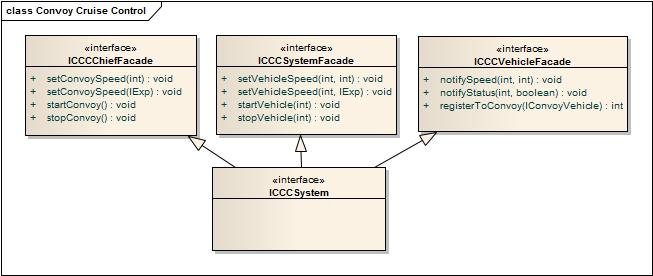
\includegraphics[scale = 0.6]{../Diagrams/Domain_Model_ICCC.jpg}\\
  \caption{Domain Model - The CCC system}\labelfig{testTypes}
\end{figure}
{\small Note how the notion of expression as a speed representation (\emph{IExp}) is present only at the boundary that forms the chief interface to the CCC.}


\subsubsection{The Convoy} $\\$
It's a line of vehicles.
%The vehicles can move while keeping a precise position in the line.
\begin{figure}
   \centering
   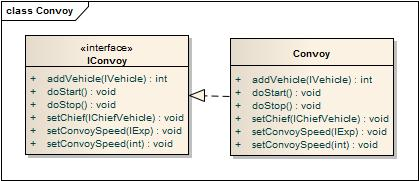
\includegraphics[scale = 0.6]{../Diagrams/Domain_Model_Convoy.jpg}\\
  \caption{Domain Model - The Convoy}\labelfig{testTypes}
\end{figure}

For a semantic description of this entity, look at the \emph{TestConvoy} test case.

\subsubsection{The Convoy Vehicle} $\\$
The vehicle is an \emph{active} entity. \newpage
\begin{figure}
   \centering
   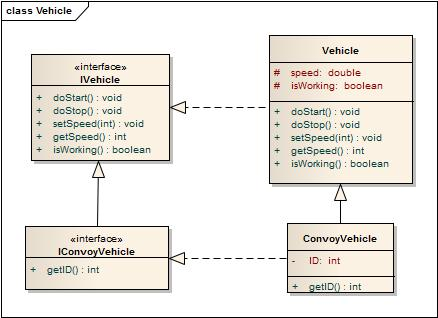
\includegraphics[scale = 0.5]{../Diagrams/Domain_Model_Vehicles.jpg}\\
  \caption{Domain Model - Vehicles}\labelfig{testTypes}
\end{figure}

\begin{figure}
   \centering
   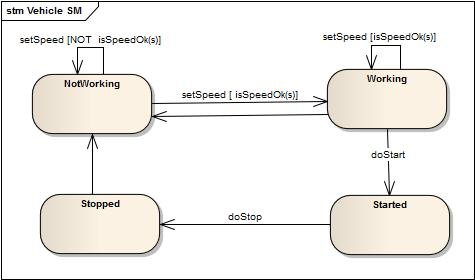
\includegraphics[scale = 0.5]{../Diagrams/Domain_Model_Vehicle-Behavioral.jpg}\\
  \caption{Domain Model - Behavioral - Vehicles}\labelfig{testTypes}
\end{figure}

For a semantic description of this entity, look at the \emph{TestVehicle} test case.

\subsubsection{The Chief Vehicle} $\\$

The chief vehicle is just a vehicle. \\ In addition, it is equipped with a dashboard that allows it to interface the chief with the CCC.

%
%\begin{figure}
%   \centering
%   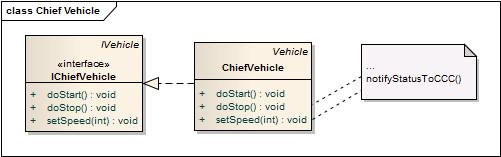
\includegraphics[scale = 0.5]{../Diagrams/Domain_Model_ChiefVehicle.jpg}\\
%  \caption{Domain Model - Chief Vehicle}\labelfig{testTypes}
%\end{figure}

%For a semantic description of this entity, look at the \emph{TestChiefVehicle} test %case.


\subsubsection{Dashboard, Display, Command Panel, Kilometer Counter, Expression Parser and Evaluator} $\\$

The Display and Kilometer Counter entities has been already modelled in a previous project ( see \emph{The Kilometer Counter} ).$\\$
The same argument applies for the dashboard (which is a frame that is able to host multiple displays and buttons), the command panel, the I/O communication infrastructure, the expression parser and evaluator.$\\$

We'll leverage on these well-proved solutions in order to strike down the cost and time of the project.


\newpage
%===========================================================================
\section{Problem analysis}
\labelsec{ProblemAnalysis}
%===========================================================================

\subsection{Main Issues}

\subsubsection{Convoy construction} $\\$
A \emph{Convoy} is composed of at least two \emph{Vehicle}, with the first one being the chief. \\
A subsequent issue regards \emph{how} a \emph{Vehicle} becomes part of the \emph{Convoy}. It may be considered a sort of registration mechanism handled through the \emph{CCC} system.

\subsubsection{Vehicle Identification} $\\$
The \emph{Vehicle}s \emph{and} their position need to be identified.\\
For example, as the speed/status information can be sent to the \emph{CCC} from different \emph{Vehicle}s, a way for discriminating between them is needed. 

% SECURITY ISSUES ????

\subsubsection{Convoy Management} $\\$
Some issues need to be considered when it has to do with the management of the \emph{Convoy}.

\begin{itemize}
  \item When a \emph{Convoy} has to be started, the vehicles must start leaving a security distance of \emph{DD} m.
  \item When a \emph{Convoy} has to be started or stopped, the \emph{CCC} and/or the \emph{Vehicle}s must guarantee that no crash happens.
\end{itemize}
It follows that a sort of \emph{reliability} is needed. \\
In particular:
\begin{itemize}
  \item A \emph{Vehicle} cannot start if the next \emph{Vehicle} hasn't started. It also has to start in order to keep the agreed security distance.
  \item A \emph{Vehicle} cannot stop if the previous \emph{Vehicle} hasn't stopped.
\end{itemize}

Some possible solutions \emph{might} include:
\begin{itemize}
  \item Sending the \emph{Start} command from the first \emph{Vehicle} to the last one, spaced with a delay that allows to guarantee the security distance;
  \item Sending the \emph{Stop} command from the last \emph{Vehicle} to the first one in order to avoid pile-up crashes;
  \item Delegating the security distance guarantee to \emph{Vehicle}s;
\end{itemize}
but it turns out that, in the first two cases, we must be sure that the command will be executed.
\\It follows that, unless abnormal situations aren't handled by the vehicles' operator, a cooperation of the \emph{Vehicle}s with the \emph{CCC} is necessary.


\subsection{Distribution}
The \emph{Convoy Cruise Control} is intrinsically a distributed system. Consequently, the notion of \emph{CCC} is distributed along the system: the \emph{Vehicle}s and the \emph{Chief Vehicle} has to be aware of it, at two distinct levels (see \emph{Fig. 2}).\\\\
As a consequence, a communication infrastructure must be up and running.\\\\
We can note also how the idea of a \emph{Convoy} as a simple aggregation of \emph{Vehicle}s is not much significant. It gets meaning when it becomes intimately related with the \emph{CCC}.

\subsection{Communication between the \emph{Vehicle}s and the \emph{CCC}}
The \emph{Vehicle}s and the \emph{Convoy Cruise Control} need to communicate. The \emph{CCC} sends commands (set speed, start, stop) to the \emph{Vehicle}s, and the \emph{Vehicle}s notify their status and speed, periodically.\\
The nature of the messages is fundamentally \emph{asynchronous}.\\\\
In addition, as we are in a distributed context, we must consider a series of issues:
\begin{itemize}
  \item We're not sure that a message will be correctly delivered to the destination;
  \item If we don't resort to an acknowledge/reply mechanism, we're also not sure if the message will be correctly executed;
  \item Timing issues raise;
  \item Security issues raise;
\end{itemize}


%We need to consider the time factor and the countless scenarios of message exchange.

%\subsection{Vehicles as observable entities}
%So that the vehicles must include a dashboard with a kilometer counter and displays which show the speed, we may opt to make them \emph{observable} entities. 

\newpage
\subsection{Logical Architecture}

\subsubsection{Interaction View} $\\$
\begin{figure}
   \centering
   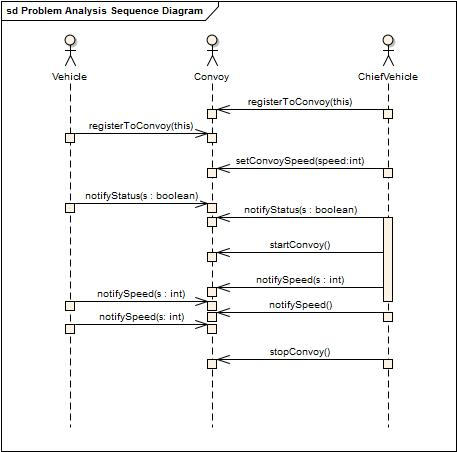
\includegraphics[scale = 0.65]{../Diagrams/Problem_Analysis_Sequence_Diagram.jpg}\\
  \caption{Logical Architecture - Interaction View}\labelfig{testTypes}
\end{figure}

\newpage

\subsubsection{Structural View} $\\$

\begin{figure}
   \centering
   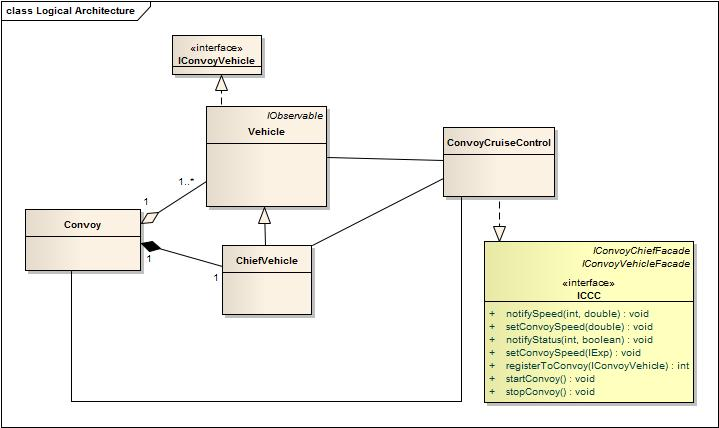
\includegraphics[scale = 0.6]{../Diagrams/Logical_Architecture.jpg}\\
  \caption{Logical Architecture - Structural View}\labelfig{testTypes}
\end{figure}




\newpage

%===========================================================================
\section{Project}
\labelsec{Project}
%===========================================================================

First of all, let's underline the main project choices and characteristics of the solution.
\begin{itemize}
  \item The \emph{Convoy} collapsed into the notion of \emph{Convoy Cruise Control} as a system. In fact, the \emph{Vehicle} and the \emph{Chief Vehicle} are more concerned with the \emph{CCC} than with the \emph{Convoy} (actually they're not concerned with the \emph{Convoy} at all once that the registration to the \emph{Convoy} is handled by the \emph{CCC}), which is hidden by the former. \\

  \item The system-wide information is placed in a centralized knowledge (data) base.\\

  \item The communication between the \emph{CCC} and the \emph{Vehicle}s can be seen as an exchange of messages and commands. So, the solution (around the \emph{IActivity} interface) is inspired to the \emph{Command} and \emph{Interpreter} patterns.\\

  \item The \emph{Vehicle}s has been made \emph{Observable} entities, so that we can attach \emph{Observer}s (such as \emph{Display}s).\\

  \item The \emph{CCC} can be seen as a sort of \emph{Observer}, so that it has to be notified for the speed and status change by the \emph{Vehicle}s.\\

  \item The sender on the client (vehicle) side and the sender/receiver on the server (chief) side are based on the \emph{Proxy} pattern.
\end{itemize}

\newpage
\subsection{Structure}

\begin{figure}
   \centering
   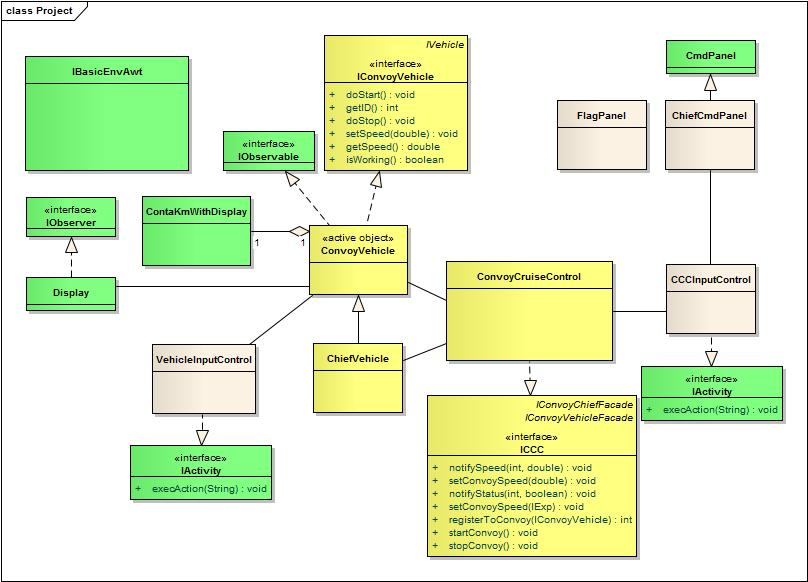
\includegraphics[scale = 0.5]{../Diagrams/Project_Structure.jpg}
  \caption{Project - Structural View}\labelfig{testTypes}
\end{figure}


\newpage
\subsection{Interaction}
\subsubsection{Vehicle to CCC}$\\$
\begin{figure}
   \centering
   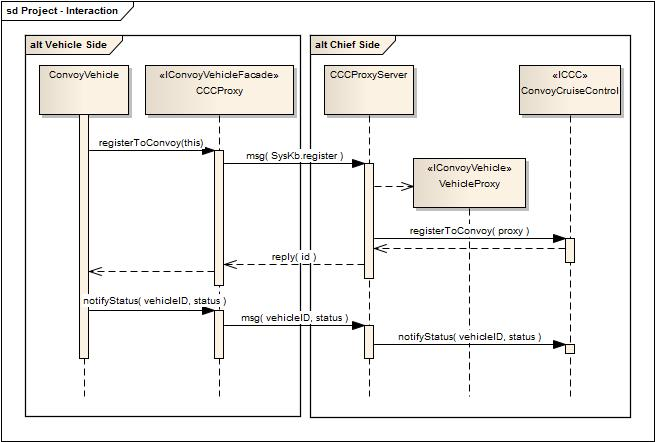
\includegraphics[scale = 0.7]{../Diagrams/Project_Interaction_VehicleToCCC.jpg}
  \caption{Project - Interaction View (Vehicle to CCC)}\labelfig{testTypes}
\end{figure}

\newpage
\subsubsection{CCC to Vehicles}$\\$
\begin{figure}
   \centering
   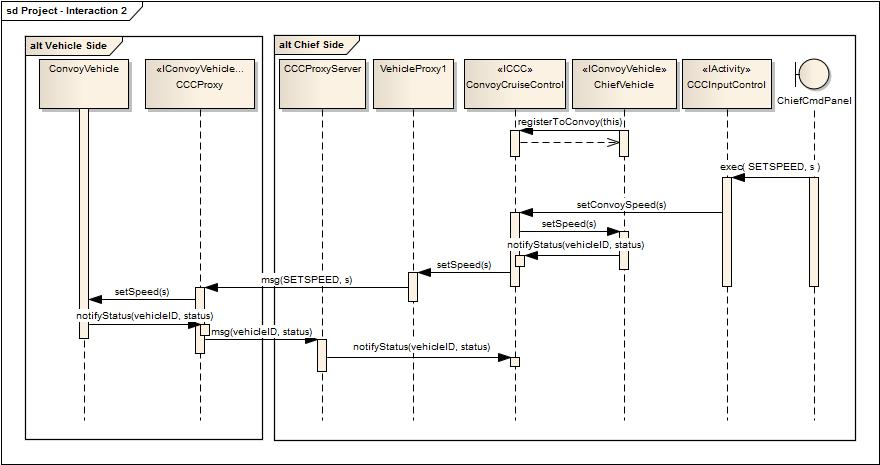
\includegraphics[scale = 0.5]{../Diagrams/Project_Interaction_CCCtoVehicles.jpg}
  \caption{Project - Interaction View (CCC to Vehicles)}\labelfig{testTypes}
\end{figure}


\newpage
%===========================================================================
\section{Implementation}
\labelsec{Implementation}
%===========================================================================
The project is implemented in the Java language as a set of Eclipse plugins (OSGI bundles).

\subsection{Component System}
\begin{figure}
   \centering
   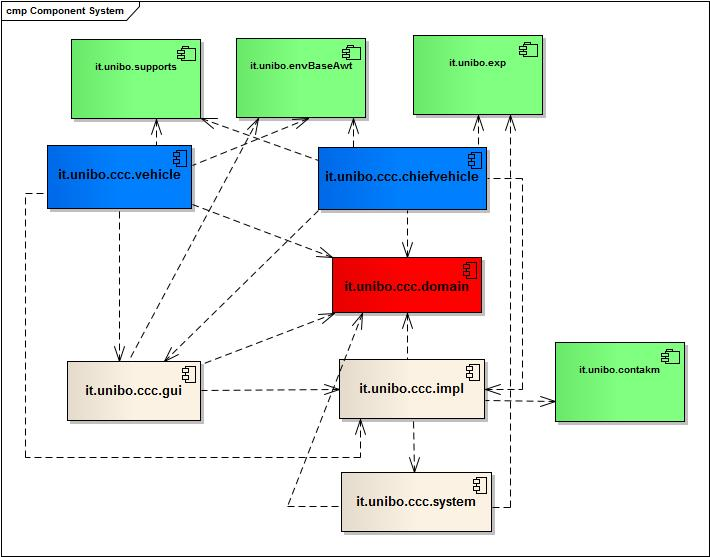
\includegraphics[scale = 0.6]{../Diagrams/Impl_Component_Structure.jpg}
  \caption{Component Dependencies Structure}\labelfig{testTypes}
\end{figure}


\newpage
%===========================================================================
\section{Deployment}
\labelsec{Deployment}
%===========================================================================
 
So that the project has been developed as a set of components represented by Eclipse plugins (OSGI bundles), it can be deployed as a set of JARs to be run on an OSGI container.

\begin{lstlisting}[label=some-code,caption=OSGI bundle installation]

> install file:plugins/it.unibo.basicInterfaces_1.4.4.jar
> install file:plugins/it.unibo.system_1.0.0.jar
> install file:plugins/it.unibo.supports_1.0.0.jar
> install file:plugins/it.unibo.envBaseAwt_1.4.4.jar

> install file:plugins/it.unibo.contaKm.displayAwt_1.0.0.jar
> install file:plugins/it.unibo.contaKm.domain_1.0.0.jar

> install file:plugins/it.unibo.exp.interfaces_1.0.0.jar
> install file:plugins/it.unibo.exp.interpreter_1.0.0.jar
> install file:plugins/it.unibo.exp.lexer_1.0.0.jar
> install file:plugins/it.unibo.exp.parser_1.0.0.jar
> install file:plugins/it.unibo.exp.token_1.0.0.jar
> install file:plugins/it.unibo.exp.expr_1.0.0.jar
> install file:plugins/it.unibo.exp.input_1.0.0.jar

> install file:plugins/it.unibo.ccc.domain_1.0.0.jar
> install file:plugins/it.unibo.ccc.system_1.0.0.jar
> install file:plugins/it.unibo.ccc.gui_1.0.0.jar
> install file:plugins/it.unibo.ccc.impl_1.0.0.jar
> install file:plugins/it.unibo.ccc.vehicle_1.0.0.jar
> install file:plugins/it.unibo.ccc.chiefvehicle_1.0.0.jar
\end{lstlisting}

Next, the bundle related to \emph{it.unibo.ccc.chiefvehicle} (chief side) and \emph{it.unibo.ccc.vehicle} (vehicle side) can be started.

\newpage
\subsection{Full Dependency Graph}

\begin{figure}
   \centering
   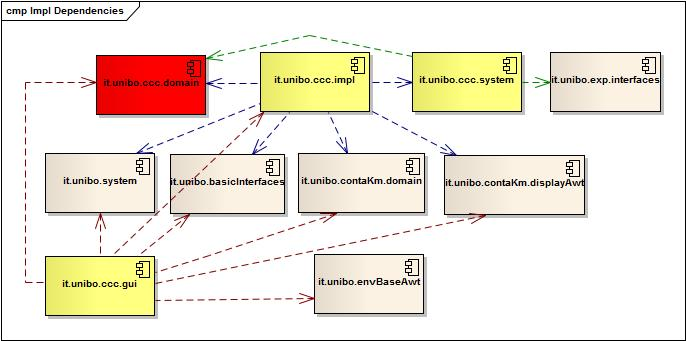
\includegraphics[scale = 0.42]{../Diagrams/Deploy_FullDep1.jpg}
  \caption{Full Dependency Graph 1}\labelfig{testTypes}
\end{figure}
\begin{figure}
   \centering
   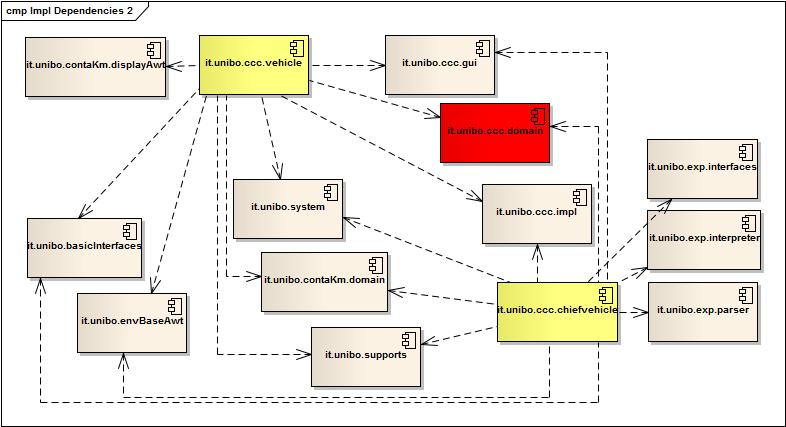
\includegraphics[scale = 0.42]{../Diagrams/Deploy_FullDep2.jpg}
  \caption{Full Dependency Graph 2}\labelfig{testTypes}
\end{figure}

%\newpage
%===========================================================================
%\section{Notes (outside the template)}
%\labelsec{Notes}
%===========================================================================
%We report here some general consideration for the next lab:
%\begin{itemize}
%  \item The solution to a problem defines \textbf{\emph{how}} we achieve some goal (how we design and implement a software system that satisfies the requirements).
%  \item Before presenting \emph{how} we achieve a goal, we must explicitly define \textbf{\emph{what}} must be achieved.
%  \item If we want to verify that our code works as it is expected, we must define \emph{what is expected} (e.g. by means of a set of \emph{testing plan}).
%  \item  To be sure that all the tests are performed, all the test should be done in \emph{automatic} way each time we modify the code.
% \end{itemize}

\newpage
%===========================================================================
\section{Testing}
\labelsec{testing}
%===========================================================================
The bundle \emph{it.unibo.ccc.tests} contains some unit tests born from the test plans for the domain entities.\\\\
A simulation can be performed by starting the bundles \emph{it.unibo.ccc.chiefvehicle} and \emph{it.unibo.ccc.vehicle}s on different machines. This can tests the functional aspects of the \emph{Convoy Cruise Control system}.\\\\
Later we'll perform an Acceptance Testing session... \\\\

%\begin{itemize}
%  \item \emph{Black box testing}: testing on the target public API without knowledge of the target source code
%  \item \emph{White box testing}: testing with knowledge of the target source code
%\end{itemize}

%\begin{figure}
%    \centering
%   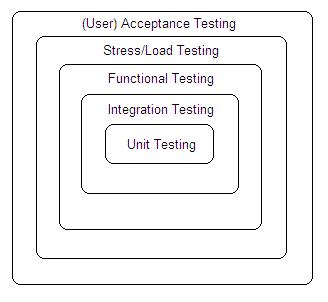
\includegraphics[scale = 0.7]{img/tests.JPG}\\
%  \caption{Test types}\labelfig{testTypes}
%\end{figure}

%\begin{itemize}
%  \item \emph{Unit Testing}: testing single units of work
%  \item \emph{Integration Testing}: testing how different units of work interact
%  \item \emph{Functional Testing}: testing subsystems (usually on a boundary API)
%  \item \emph{Stress/Load Testing}: testing the system performance
%  \item (\emph{User) Acceptance Testing}: testing the system as a user
%\end{itemize}





\appendix


\bibliographystyle{abbrv}
%\bibliography{biblio}

\end{document}












